%In this section we firstly discuss relative entropy regularization for policy based reinforcement learning and its relationship with mirror descent, paving the path for presenting our proposed Reversed Entropy Policy Mirror Descent (REPMD) algorithm. 
In this section, we first present our algorithm PMD.
As mentioned in \cref{sec:intro}, we focus on analyzing its properties in the \emph{non-convex} setting.
Two additional modifications are then proposed in \cref{subsec:repmd}, leading to our main algorithm REPMD.
Lastly, although our algorithm is developed purely policy-based, it can be easily extended to cooperate with value function approximation. 
We briefly discussed the actor-critic version of our method in \cref{subsec:repmd_value}.
\if0
Our first algorithm, Policy Mirror Descent (PMD), is derived from the basic idea of maximizing the relative entropy-regularized expected reward. Such objective has also been used in various reinforcement learning algorithms including \citet{williams1991function,fox2015taming,schulman2017equivalence,nachum2017bridging,haarnoja2017reinforcement}, among others.
As mentioned in \cref{sec:intro}, we focus on analyzing its learning properties in the \emph{non-convex} setting in parameter space.
Our first step in \cref{subsec:revisitTRPO} is to reformulate the 
objective as a lift-and-project procedure following the idea of Mirror Descent. 
We discuss the properties and potential deficiencies of PMD based on such reformulation.
Additional modifications are then proposed  to mitigate these deficiencies in \cref{subsec:repmd}, leading to a new algorithm called Reversed Entropy Policy Mirror Descent (REPMD).
As we will see in \cref{subsec:repmd,subsec:sr}, REPMD enjoys some performance guarantees even in the non-convex setting, e.g. when $\pi_\theta$ is an one-layer-softmax neural network. 
Lastly, although our algorithm is presented purely policy-based, it can be easily extended to cooperate with value function approximation. 
We briefly discussed the actor-critic version of our method in \cref{subsec:repmd_value}.

\subsection{Policy Mirror Descent}
\label{sec:pmd}
We first present a basic policy optimization algorithm based on the idea of Mirror Descent (MD). MD has been widely used in the literature of online learning and constrained optimization problems \citep{nemirovskii1983problem,beck2003mirror}. In particular, given a \emph{reference policy} $\refPi$, let 
\begin{equation*}
\ENT(\pi_\theta; \tau, \refPi) = { \ep\limits_{\rho \sim \pi_\theta}{  r(\rho)  - \tau \KL(\pi_\theta \| \refPi) } }.
\end{equation*}

The MD update for policy optimization problem is 
\begin{equation}
%\label{eq:max_expected_reward_plus_relative_entropy}
\pi_{\theta_{t+1}} = \argmax\limits_{\pi_\theta \in \Pi}  \ENT(\pi_\theta; \tau, \pithetat), 
\end{equation}
which combines the expected reward \cref{max_expected_reward} with a relative entropy regularizer. Similar ideas have also been explored in \citet{peters2007reinforcement,wierstra2008episodic,peters2010relative,schulman2015trust,montgomery2016guided,nachum2017trust,haarnoja2018soft,abdolmaleki2018maximum}. The following \cref{prop:mirrordescent_projection} suggests an efficient implementation of the mirror descent algorithm.
Based on \cref{prop:mirrordescent_projection}, policy mirror descent (PMD) updates the policy $\pi_{\theta_{t+1}}$ by
\begin{equation}
%\label{eq:pmd}
\begin{split}
&\argmin\limits_{\pi_\theta \in \Pi}{\KL( \pi_\theta \| \bar{\pi}_{\tau}^* )}, \\
\text{where}\ \ \bar{\pi}_{\tau}^* & =  \argmax\limits_{\pi \in \Delta}{ \ep\limits_{\rho \sim \pi}{  r(\rho)  - \tau \KL(\pi \| \pi_{\theta_t}) } }.
\end{split}
\end{equation}
\fi

\subsection{Policy Mirror Descent}
\label{subsec:revisitTRPO}
%Recall that TRPO\footnote{Here we present its regularized version, which is equivalent to constraint version that is presented in \citet{schulman2015trust}. } learns the policy by maximizing the expected reward with a relative entropy regularizer.

Given a \emph{reference policy} $\refPi$ (usually the current policy), 
an algorithm that maximizes the relative entropy regularized expected reward typically learns $\pi_{\theta} $ by 
%let 
\begin{equation}
%\ENT(\pi_\theta; \tau, \refPi) = 
\label{eq:max_expected_reward_plus_relative_entropy}
\pi_{\theta} = \argmax\limits_{\pi_\theta \in \Pi} { \ep\limits_{\rho \sim \pi_\theta}{  r(\rho)  - \tau \KL(\pi_\theta \| \refPi) } }.
\end{equation}
Besides reinforcement learning, such regularizer has been widely used in the literature of online learning and constrained optimization problems \citep{nemirovskii1983problem,beck2003mirror}, mostly in the mirror descent algorithm.
Note that when $\refPi$ is a uniform distribution, \cref{eq:max_expected_reward_plus_relative_entropy} also ensembles the entropy regularizer.
%\begin{equation}
%\label{eq:max_expected_reward_plus_relative_entropy}
%\pi_{\theta_{t+1}} = \argmax\limits_{\pi_\theta \in \Pi}  \ENT(\pi_\theta; \tau, \pithetat). 
%\end{equation}
%which combines the expected reward \cref{max_expected_reward} with a relative entropy regularizer. 
%Similar ideas have also been explored in \citet{peters2007reinforcement,wierstra2008episodic,peters2010relative,schulman2015trust,montgomery2016guided,nachum2017trust,haarnoja2018soft,abdolmaleki2018maximum}. 

To better analyze its behavior in the parameter space, in this paper we follow the idea of mirror descent to reformulate the problem as a lift-and-project procedure.
\begin{equation}
\label{eq:pmd}
\begin{split}
\text{\bf (Project Step)} \quad &\argmin\limits_{\pi_\theta \in \Pi}{\KL( \pi_\theta \| \bar{\pi}_{\tau}^* )}, \\
\text{\bf (Lift Step)}  \quad & \text{where}\ \ \bar{\pi}_{\tau}^* =  \argmax\limits_{\pi \in \Delta}{ \ep\limits_{\rho \sim \pi}{  r(\rho)  - \tau \KL(\pi \| \refPi) } }. 
\end{split}
\end{equation}
\cref{prop:mirrordescent_projection} shows that the problems of \cref{eq:pmd} and \cref{eq:max_expected_reward_plus_relative_entropy} are in fact equivalent, even when $\pi$ is non-convex in $\theta$.
Note that although it is non-convex in $\pi$ for the lift step, we can actually solve the problem analytically, where
\begin{equation}
\label{eq:pitaustar}
\bar{\pi}_\tau^*(\rho) =  \frac{\refPi(\rho) \exp\left\{ r(\rho) / \tau \right\}}{ \sum_{\rho^{\prime}}{\refPi(\rho^{\prime}) \exp\left\{ r(\rho^{\prime}) / \tau \right\} } }.
\end{equation}
\begin{prop}
\label{prop:mirrordescent_projection}
Given a \emph{reference policy} $\refPi$,
\[
 \argmax\limits_{\pi_\theta \in \Pi} { \ep\limits_{\rho \sim \pi_\theta}{  r(\rho)  - \tau \KL(\pi_\theta \| \refPi) } } 
 = \argmin\limits_{\pi_\theta \in \Pi}{ \KL(\pi_\theta \| \bar{\pi}_\tau^*) }.
\]
\end{prop}
%\begin{remk}
%	The lift-and-project procedure in \cref{eq:pmd} is not completely new in the literature. In fact, it has also been proposed in \cite{montgomery2016guided,tangkaratt2017guide,abdolmaleki2018maximum,haarnoja2018soft}. We postpone the comparison between our method and theirs to \cref{sec:related_work}.
%\end{remk}

The lift-and-project reformulation suggests an alternative algorithm: Lift the current policy $\pi_{\theta_t}$ to $\bar{\pi}_\tau^*$, then perform multiple steps of gradient descent on the project step to update $\pi_{\theta_{t+1}}$. \footnote{To estimate this gradient, one would need to use the self-normalized importance sampling \cite{owen2013monte}. We omit the implementation details here since PMD  is not the main algorithm of this paper.}
We name this method by Policy Mirror Descent (PMD).  \todor[]{May wanna add the implementation details in Appendix.}
%Note that vanilla gradient descent methods for TRPO can be interpreted as performing only one step gradient descent for the project step. \todor[]{Is it correct?} 
One can show that PMD asymptotically converges to the optimal policy when $\Pi$ is a convex set \citep{nemirovskii1983problem,beck2003mirror}. 
%However, in practice, the policy $\pi_\theta$ is often parameterized by a complex non-convex function, such as a neural network, which violates the convex constraint set assumption. 
The next proposition shows that despite of the non-convexity of $\Pi$, PMD still has some desirable properties.
\begin{prop}
\label{prop:monoto_policymirrordescent}
Given the project step $\min\limits_{\pi_\theta \in \Pi}{\KL( \pi_\theta \| \bar{\pi}_{\tau}^* )}$ can be solved globally optimally, PMD satisfies the following properties for an arbitrary parametrization of $\pi$.
\begin{enumerate}
	\item {\bf (Monotonic Improvement Guarantee)} 
	%The sequence of policies learned by TRPO is guaranteed to be monotonically improved:
	Assume that $\pi_{\theta_{t}}$ is the update sequence, then 
	 \begin{equation*}
	\oep_{\rho \sim \pi_{\theta_{t+1}}}{r(\rho)} - \oep_{\rho \sim \pi_{\theta_{t}}}{  r(\rho)} \ge 0.
	\end{equation*}
	\item {\bf (Global optimum inclusion)} Every stationary point of the expected reward $\oep_{\rho \sim \pi_\theta}{  r(\rho)}$, including the globally optimal policy $\pi_{\theta^*}$,  is a fixed point of PMD.
	%The globally optimal policy $\pi^*$ in parameter space is included in the set of fixed points of TRPO.
\end{enumerate}
\end{prop}

%\begin{remk}
%	The monotonic improvement guarantee has been derived in \citep{schulman2015trust}. We give a simpler and direct proof based on our lift-and-project formulation in \cref{appsec:monoto_policymirrordescent} .
%\end{remk}
Despite of the desirable properties, 
\cref{prop:monoto_policymirrordescent}
%Another problem about TRPO is that \cref{prop:monoto_policymirrordescent} 
relies on the condition that the projection step of PMD needs to be globally optimally solved.
Oftentimes in practice this is not true when $\pi_\theta$ is non-convex in $\theta$, which hinders the applicability of \cref{prop:monoto_policymirrordescent}.

Another problem is that PMD is observed to get trapped in some poor local optima in practice. 
Indeed, while the relative entropy regularizer helps in preventing large policy update, it may also limit the exploration of TRPO.
Moreover, minimizing the KL divergence $\KL(\pi_\theta \| \bar{\pi}_\tau^*) $ is known to be \emph{mode seeking} \citep{kevin2012machine}, which can cause mode collapse during the learning process. Once the policy $\bar{\pi}_\tau^*$ drops some of the modes, learning could be trapped into sub-optimal policies.
At this point, the relative entropy regularizer will NOT encourage PMD for further exploration.



\subsection{Reversed Entropy Policy Mirror Descent}
\label{subsec:repmd}
\if0 
First, an additional entropy regularizer, controlled by a separate parameter $\tau^{\prime}\geq 0$, is added to the objective, which encourages additional exploration as in MENT.

A similar monotonic improvement result to \cref{prop:monoto_policymirrordescent} can also be proved for REPMD but only on the $\SR(\pi_\theta) $, as shown in \cref{thm:monotonically_increasing_sr_property}, where we let
\begin{equation*}
\SR(\pi_\theta) \triangleq (\tau + \tau^{\prime})\log{ \sum_{\rho}{ \exp\left\{ \frac{r(\rho) + \tau \log{\pi_\theta(\rho)} }{\tau + \tau^{\prime}} \right\} }}
\end{equation*}
denote the softmax approximated expected reward of $\pi_\theta$.
\fi
In this section, we propose two modifications to PMD to overcome its aforementioned potential deficiencies.
The first modification is an additional entropy regularizer to the lift step, controlled by a separate parameter $\tau^{\prime}\geq 0$, to encourage the exploration of the algorithm. 
Second, we employ the reversed \emph{mean seeking} direction of KL divergence, $\KL(\bar{\pi}_{\tau,\tau^{\prime}}^* \| \pi_\theta)$, for the project step.
The new algorithm, called Reversed Entropy Policy Mirror Descent (REPMD), solves the following optimization problem to update the policy $\pi_{\theta_{t+1}}$:
\begin{equation}
\label{eq:repmd}
\begin{split}
\text{\bf (Project Step)} \quad  &\argmin\limits_{\pi_\theta \in \Pi}{\KL(\bm{ \bar{\pi}_{\tau,\tau^{\prime}}^* \| \pi_\theta }) }, \\
\text{\bf (Lift Step)} \quad  & \text{where}\ \ \bar{\pi}_{\tau,\tau^{\prime}}^*  =  \argmax\limits_{\pi \in \Delta}{ \ep\limits_{\rho \sim \pi}{  r(\rho)  - \tau \KL(\pi \| \pi_{\theta_t}) + \bm{\tau^{\prime} \cH(\pi)} }}.
\end{split}
\end{equation}
%, leading to our new algorithm.
The idea of optimizing the reverse direction of KL divergence has proven to be effective for structured prediction and reinforcement learning in previous work, such as reward augmented maximum likelihood \citep{norouzi2016reward} and UREX \citep{nachum2017improving}.
Its \emph{mean seeking} behavior would further encourage the exploration of the algorithm.

As we will see in \cref{sec:experiments}, REPMD outperforms PMD significantly in our experiments. 
\cref{thm:monotonically_increasing_sr_property} further shows that REPMD also enjoys similar desirable properties, but on a surrogate reward $\SR(\pi_\theta) $.
\begin{thm}
\label{thm:monotonically_increasing_sr_property}
Given the project step $\KL( \bar{\pi}_{\tau,\tau^{\prime}}^* \| \pi_\theta )$ can be solved globally optimally, REPMD satisfies the following properties for an arbitrary parametrization of $\pi$.
\begin{enumerate}
	\item {\bf (Monotonic Improvement Guarantee)} 
	%The sequence of policies learned by TRPO is guaranteed to be monotonically improved:
	Assume that $\pi_{\theta_{t}}$ is the update sequence, then 
	\begin{equation*}
	\SR(\pi_{\theta_{t+1}}) - \SR(\pithetat)\ge 0,
	\end{equation*}
	where
	\begin{equation}
	\label{eq:SR}
	\SR(\pi_\theta) \triangleq (\tau + \tau^{\prime})\log{ \sum_{\rho}{ \exp\left\{ \frac{r(\rho) + \tau \log{\pi_\theta(\rho)} }{\tau + \tau^{\prime}} \right\} }}.
	\end{equation}
	\item {\bf (Global optimum inclusion)} Every stationary point of the expected reward $\text{SR}(\pi_\theta)$, including the globally optimal policy $\pi_{\theta^*}$,  is a fixed point of REPMD. \todor[]{Double check} \todoj[]{Add proof in A.3}
	%The globally optimal policy $\pi^*$ in parameter space is included in the set of fixed points of TRPO.
\end{enumerate}
%Theorem \ref{thm:monotonically_increasing_sr_property} guarantees the monotonic improvement on $\text{SR}(\pi)$, thus implies that 
the fixed points of REPMD have a correspondence with the stationary point of $\text{SR}(\pi_\theta)$. \todor[]{Why?}
\end{thm}

Furthermore, as shown in \cref{prop:solvableprojection}, 
for the one-layer-softmax neural network $\pi$, the condition in \cref{thm:monotonically_increasing_sr_property}, that $\KL( \bar{\pi}_{\tau,\tau^{\prime}}^* \| \pi_\theta )$ can be solved globally optimally, can now be satisfied in practice.
%reversing the direction of the KL divergence makes the projection step solvable even for the one-layer-softmax neural network $\pi$, thus guarantees the desirable properties in practice.
\begin{prop}
	\label{prop:solvableprojection}
	Assume $\pi_\theta(s) = \softmax(\phi_s^{\top}\theta)$. Given a reference policy $\refPi$, the projection step $\min\limits_{\theta \in \mathbb{R}^d}{\KL(\refPi \| \pi_\theta)}$ is convex in $\theta$.
\end{prop}


\subsubsection{Behavior of $\SR(\pi)$}
\label{subsec:sr}
Although $\text{SR}(\pi_\theta)$ is different from the expected reward $\ep_{\rho \sim \pi_\theta}{r(\rho)}$,  in this section we present some theoretical and empirical evidences that $\SR(\pi_\theta)$ is a reasonable surrogate that may provide good guidance to the learning. 
In fact, by properly adjusting the two temperature parameters $\tau$ and $\tau^{\prime}$, $\SR(\pi_\theta)$ recovers several existing performance measures, as shown in \cref{prop:sr}.
\begin{prop}
\label{prop:sr}
$\SR(\pi_\theta)$ satisfies the following properties:
\begin{enumerate}[label=(\roman*)]
	\item  $\SR(\pi_\theta) \to \max_{\rho}{r(\rho)}$, as $\tau \to 0, \tau^{\prime} \to 0$.
	\item $\SR(\pi_\theta) \to \ep_{\rho \sim \pi_\theta}{r(\rho)}$, as $\tau \to \infty, \tau^{\prime} \to 0$. 
\end{enumerate}	
\end{prop}
\begin{remk}
	Note that $\text{SR}(\pi_\theta)$ also resembles ``softmax value function'' that appeared in value based RL \citep{nachum2017bridging,haarnoja2018soft,ding2017cold}. The standard soft value can be recovered by $\text{SR}(\pi_\theta)$ as a special case when $\tau = 0$ or $\tau'=0$. 
	%\todor[]{But \cref{prop:sr} says that $SR(\pi)$ converges to $max_\rho$ when $\tau$ and $\tau^\prime$ are 0?}
\end{remk}

\begin{wrapfigure}{r}{0.56\textwidth}
	\begin{minipage}{0.56\textwidth}
		\begin{algorithm}[H]
			\caption{\label{alg:repmd}  The REPMD algorithm}
			\begin{algorithmic}[1]
				\INPUT $\tau, \tau', K$
				\OUTPUT  Policy $\pi_\theta$
				\STATE Random initialized $\pi_{\theta_1}$;
				\FOR { $t=1,2,\ldots, T$ }
				\STATE Set $\refPi = \pithetat$;
				\REPEAT 
				\STATE Sample a mini-batch of $K$ trajectories from $\refPi$;
				\STATE Compute the gradient according to \cref{eq:gradient_estimator};
				\STATE Update $\pi_{\theta_{t+1}}$ by the gradient;
				\UNTIL converged or reach max\_iter;
				\ENDFOR
				\STATE Return $\pi_{\theta_T}$.
			\end{algorithmic}
		\end{algorithm}
	\end{minipage}
\end{wrapfigure}

According to \cref{prop:sr}, one should gradually decrease $\tau^{\prime}$ to reduce the level of exploration as sufficient reward landscape information has been collected during the learning process. Now we can make different choices for $\tau$, depending on the policy constraint set $\Pi$.
%\begin{remk}
%\label{small_tau_choices}
Given $\tau^{\prime} \to 0$ and the reward landscape has been sufficiently explored,
the constructed unconstrained policy $\bar{\pi}_{\tau,\tau^{\prime}}^* \to \pi^*$ as $\tau \to 0$, where $\pi^*$ is the global deterministic optimal policy. 
Therefore, in the project step $\pi_\theta$ is obtained by directly projecting $\pi^*$ into $\Pi$. When the policy constraint $\Pi$ has nice properties, such as convexity, that support good behavior of KL projection, $\pi_\theta$ may achieve good performance.
However, in practice, $\Pi$ is typically non-convex. Setting $\tau \to 0$ might not work very well, since directly projecting $\pi^*$ into $\Pi$ does not always lead to a $\pi_\theta$ with large expected reward.

On the other hand, as $\tau \to \infty$ the stationary point set of $\SR(\pi_\theta)$ will approach the stationary point set of $\sum_{\rho}{ \pi_\theta(\rho) r(\rho) }$.
There exists an ideal sequence of $\tau$ values and $\tau \to \infty$ that make $\pi_\theta$ finally converge to $\pi_\theta^* \in \argmax_{\pi_\theta}{ \sum_{\rho}{\pi_\theta(\rho) r(\rho)} }$, i.e., the optimal policy in $\Pi$ with highest expected reward, recovering the target of policy optimization \cref{max_expected_reward}. \todor[]{Why?}
We empirical investigate the behavior of $\SR{\pi}$ on a simulation setting, as shown in \cref{fig:srsimulation}.
\todor[]{Add the simulation setting in the caption of the figure.}
Note that there is a poor local maximum for $\theta <0$, where naive gradient method will converge to if $\theta$ is initialized on the left. 
Picking $\tau = 0.2$, the reward landscape of $SR(\pi)$ guides $\theta$ to converges the neighbourhood of $0$, avoiding such poor local maximum. Later in the training when $\tau$ increases to $10$, $SR(\pi)$ recovers the true expected reward landscape, where $\theta$ will converge to good local , if not the global, maximum.
While a simulation result may be still preliminary, it suggests that $\SR(\pi)$ could be a good guidance for maximizing the true expected reward in some cases.
Further investigation and a principled way to find such an ideal sequence of $(\tau,\tau')$ is left for future work.
 \todor[]{Add the simulation result for true loss and $\SR(\pi)$ with different value of $\tau$.}
\if0
Using very small $\tau$ value, i.e., $\tau \to 0$, given $\tau^{\prime} \to 0$ and the reward landscape has been sufficiently explored, the constructed unconstrained policy $\bar{\pi}_{\tau,\tau^{\prime}}^* \to \pi^*$, where $\pi^*$ is the global deterministic optimal policy. Solving the projection $\pi_\theta \leftarrow \argmin_{\pi_\theta \in \Pi}{\KL(\bar{\pi}_{\tau,\tau^{\prime}}^* \| \pi_\theta}) \approx \argmin_{\pi_\theta \in \Pi}{\KL(\pi^* \| \pi_\theta})$, we actually obtain $\pi_\theta$ policy by directly projecting $\pi^*$ into $\Pi$. When the policy constraint $\Pi$ has additional nice properties, such as convexity, that support good behavior of KL projection, this should be a good choice.
%\end{remk}
However, in practice, $\Pi$ is typically non-convex, even when $\pi_\theta$ is parameterized by a linear function approximator, let alone more complex function approximations like a neural network. In such cases, the small $\tau$ value suggested in Remark \ref{small_tau_choices} might not work very well, since directly projecting $\pi^*$ into $\Pi$ might not always lead to a $\pi_\theta$ with large expected reward.

\begin{remk}
\label{large_tau_choices}
	Given $\tau^{\prime} \to 0$ and a sufficiently explored reward landscape, as $\tau \to \infty$, the stationary point set of $\SR(\pi_\theta)$ will approach the stationary point set of $\sum_{\rho}{ \pi_\theta(\rho) r(\rho) }$.
\end{remk}
 
Remark \ref{large_tau_choices} indicates that during learning, $\pi_\theta$ may get stuck around some local maximum of $\SR(\pi_\theta)$, and increasing the $\tau$ value will lead to a different contour of $\SR(\pi_\theta)$, which might help $\pi_\theta$ escape to alternative local maxima. There exists an ideal sequence of $\tau$ values and $\tau \to \infty$ that make $\pi_\theta$ finally converge to $\pi_\theta^* \in \argmax_{\pi_\theta}{ \sum_{\rho}{\pi_\theta(\rho) r(\rho)} }$, i.e., the optimal policy in $\Pi$ with highest expected reward, recovering the target of policy optimization \cref{max_expected_reward}. A principled way to find such an ideal sequence of $\tau$ is under investigation.
 \fi
 
\begin{figure*}[t]
\begin{center}
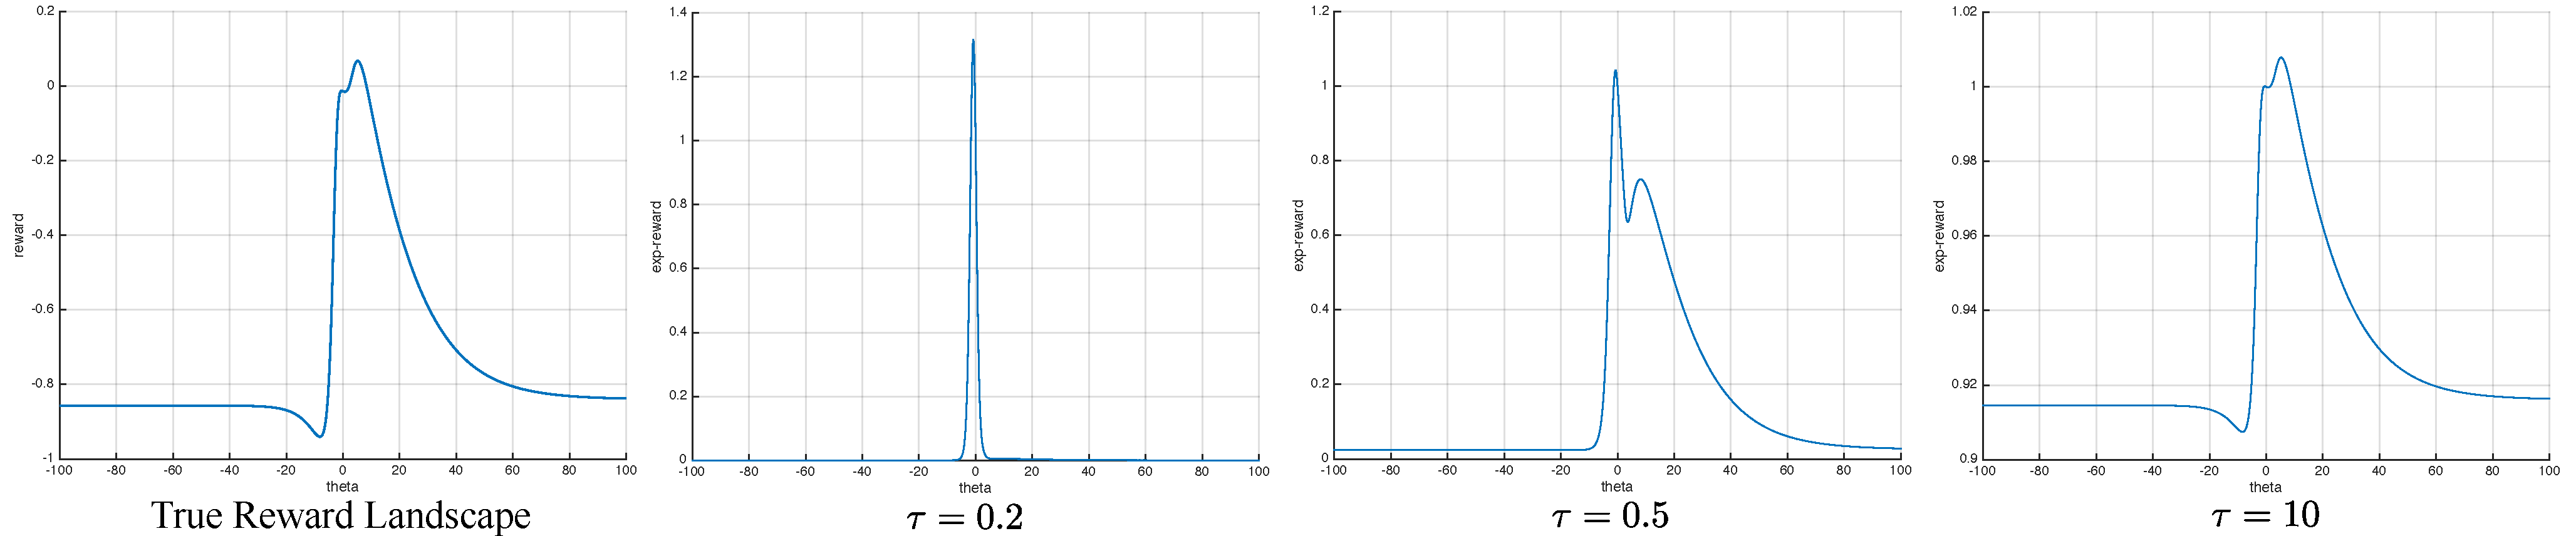
\includegraphics[width=1.0\linewidth]{./sr_simulation.pdf}
\end{center}
\caption{
Simulation result for true reward landscape and $\SR(\pi)$ with different value of $\tau$.} 
\label{fig:srsimulation}
\end{figure*}
 
\subsection{Learning}
\label{subsec:learning}
We now discuss the implementation details of REPMD. The full algorithm is presented in \cref{alg:repmd}.
Despite of its non-convexity, it can be verified that the lift step has an analytic solution
\begin{equation}
\label{eq:pitautauprime}
\bar{\pi}_{\tau,\tau^{\prime}}^*(\rho) \triangleq \frac{\refPi(\rho) \exp\left\{ \frac{r(\rho)-\tau^{\prime} \log \refPi(\rho) }{ \tau+\tau^{\prime}} \right\}}{ \sum_{\rho^{\prime}}{\refPi(\rho^{\prime}) \exp\left\{ \frac{r(\rho^{\prime})-\tau^{\prime} \log \refPi(\rho^{\prime})}{ \tau+\tau^{\prime}} \right\} } }.
\end{equation}
%First note that the \emph{unconstrained optimal policy} $\bar{\pi}_{\tau,\tau^{\prime}}^*$ in (\ref{eq:repmd}) has a closed form expression.
The project step in \cref{eq:repmd}, $\min\limits_{\pi_\theta \in \Pi}{\KL(\bm{ \bar{\pi}_{\tau,\tau^{\prime}}^* \| \pi_\theta }) }$, can be optimized via stochastic gradient descent, given that one can sample trajectories from $\bar{\pi}_{\tau,\tau^{\prime}}^*$ to estimate its gradient.
To see that, note that 
\begin{equation*}
\argmin\limits_{\pi_\theta \in \Pi}\KL(\bar{\pi}_{\tau,\tau^{\prime}}^* \| \pi_\theta) = \argmin\limits_{\pi_\theta \in \Pi} \ep_{\rho \sim \bar{\pi}_{\tau,\tau^{\prime}}^* }  - \log \pi_\theta(\rho).
\end{equation*}
The next theorem shows that sampling from $\bar{\pi}_{\tau,\tau^{\prime}}^*$ can be done using self-normalized importance sampling \citep{owen2013monte}, following the idea of UREX \citep{nachum2017improving}.
\begin{thm}
\label{thm:repmdgradientestimate}
Let $\omega_k = \frac{r(\rho_k) - \tau^{\prime} \log{\refPi(\rho_k)} }{\tau + \tau^{\prime}}$. Given $K$ \emph{i.i.d.} samples $\{\rho_1, \dots, \rho_K\}$ from the \emph{reference policy} $\refPi$, we have the following unbiased gradient estimator,
\begin{equation}
\label{eq:gradient_estimator}
	\nabla_{\theta} \KL(\bar{\pi}_{\tau,\tau^{\prime}}^* \| \pi_\theta)\approx -\sum\limits_{k=1}^K{ \frac{ \exp\left\{ \omega_k \right\} }{ \sum_{j=1}^K{ \exp\left\{ \omega_j \right\}}} \nabla_{\theta} \log{\pi_\theta(\rho_k)} },
\end{equation}
%	where 
%	\[
%	\omega_k = \frac{r(\rho_k) - \tau^{\prime} \log{\refPi(\rho_k)} }{\tau + \tau^{\prime}}.
%	\] 
\end{thm}

\subsection{Cooperate with Value Function Approximation}
\label{subsec:repmd_value}
\newcommand{\parV}{V_{\phi}}
\newcommand{\parTargetV}{V_{\bar{\phi}}}
\newcommand{\parQ}{Q_{\psi}}
\newcommand{\parPi}{\pi_{\theta}}
\newcommand{\parQone}{Q_{\psi_1}}
\newcommand{\parQtwo}{Q_{\psi_2}}

%We consider an infinite trajectory $\rho$ while keeping the discounted factor $\gamma=1$ for simplicity. All the results have no difficulty to extend to a  general value of $\gamma$. 
Given a reference policy $\refPi$ and an initial state $s$, recall that the objective in the lift step is 
\[
\gO_{\text{REPMD}}(\pi, s) =   \ep\limits_{\rho \sim \pi}{  r(\rho)  - \tau \KL(\pi \| \refPi) + \tau^{\prime} \cH(\pi)}, 
\]
where $\rho=  (s_1 = s, a_1, s_2, a_2, \ldots)$.
 To cooperate with value function approximation, we will need to derive the temporal consistency for this objective, as follows. 
 \[
 \gO_{\text{REPMD}}(\pi, s) = \E_{a\sim \pi(\cdot \vert s)} \left[ r(s,a) + \gO_{\text{REPMD}}(\pi, s')  + \tau \log \refPi(a|s) - \left(\tau+ \tau' \right) \log \pi(a|s) \right]. 
 \]
%We first alter our definitions of policy and value functions to include the KL and entropy regularization. Given a reference policy $\refPi(a|s)$, we consider the entropy regularized maximum reward objective, \todoc[]{add the trust-pcl reference here or just discuss it in related work?}
%\begin{equation*}
%\gO_{\text{RELENT}}(\pi, s) = \E_{a\sim \pi} \left[ r(s,a) + \gO_{\text{RELENT}}(\pi, s')  + \tau \log \refPi(a|s) - \left(\tau+ \tau' \right) \log \pi(a|s) \right] \\
%\label{relent-obj}
%\end{equation*}
Let $\bar{\pi}_{\tau,\tau^{\prime}}^* (\cdot|s) = \argmax_{\pi} \gO_{\text{REPMD}}(\pi, s) $ denote the optimal policy on state $s$. 
%By \cref{eq:pitautauprime}, 
%\[
%\bar{\pi}_{\tau,\tau^{\prime}}^* (a|s) = \frac{1}{Z} \exp \left\{ \frac{\left[ r(s,a) + \gO_{\text{REPMD}}(\bar{\pi}_{\tau,\tau^{\prime}}^* (\cdot|s'), s') \right] + \tau \log \bar{\pi}(a|s) }{\tau + \tau'} \right\}.
%\]
Further denote the soft optimal state value function $\gO_{\text{REPMD}}(\bar{\pi}_{\tau,\tau^{\prime}}^* (\cdot|s), s)$ by $\bar{V}_{\tau,\tau^{\prime}}^*(s)$, and let  $\bar{Q}_{\tau,\tau^{\prime}}^*(s,a) = r(s,a) + \gamma \bar{V}_{\tau,\tau^{\prime}}^*(s')$ be the soft-Q function.
 It can be verified that 
\begin{equation}
\begin{split}
& \bar{V}_{\tau,\tau^{\prime}}^*(s) = (\tau + \tau') \log \sum_a \exp \left\{ \frac{\bar{Q}_{\tau,\tau^{\prime}}^*(s,a) + \tau \log \bar{\pi}(a|s)} {\tau + \tau'} \right\}; \\
& \bar{\pi}_{\tau,\tau^{\prime}}^* (a|s) = \exp \left\{ \frac{\bar{Q}_{\tau,\tau^{\prime}}^*(s,a) + \tau \log \bar{\pi}(a|s) - \bar{V}_{\tau,\tau^{\prime}}^*(s)}{\tau + \tau'} \right\}.
\end{split}
\label{soft-v-and-pi}
\end{equation}
 
% The soft optimal state value can be defined by $\bar{V}_{\tau,\tau^{\prime}}^*(s) = \gO_{\text{RELENT}}(\bar{\pi}_{\tau,\tau^{\prime}}^*, s)$. According to \cref{eq:pitautauprime}, both $\bar{\pi}_{\tau,\tau^{\prime}}^*(\cdot | s)$ and $\bar{V}_{\tau,\tau^{\prime}}^*(s)$ have closed form solution that,

%\subsubsection{Learning}
We propose to train a soft state value function $\parV$ parameterized by $\phi$, a soft Q-function $\parQ$ parameterized by $\psi$, and a policy $\parPi$ parameterized by $\theta$, based on \cref{eq:repmd}. We now derive the update rules for these parameters. 

The soft state value function approximates the soft optimal state value $\bar{V}_{\tau,\tau^{\prime}}^*$. Note that we can re-express $\bar{V}_{\tau,\tau^{\prime}}^*$ by 
\begin{align*}
\bar{V}_{\tau,\tau^{\prime}}^*(s) 
%= & (\tau + \tau') \log \sum_a \refPi(a|s) \exp \left\{ \frac{\bar{Q}_{\tau,\tau^{\prime}}^*(s,a) - \tau' \log \bar{\pi}(a|s)} {\tau + \tau'} \right\} \\ 
= & (\tau + \tau') \log \E _ {a\sim \refPi} \left[ \exp \left\{ \frac{\bar{Q}_{\tau,\tau^{\prime}}^*(s,a) - \tau' \log \bar{\pi}(a|s)} {\tau + \tau'} \right\} \right].
\end{align*}
This suggests a Monte-Carlo estimation of $\bar{V}_{\tau,\tau^{\prime}}^*(s)$: by sampling one single action $a$ according to the reference policy $\refPi$, we have $\bar{V}_{\tau,\tau^{\prime}}^*(s) \approx  \bar{Q}_{\tau,\tau^{\prime}}^*(s,a) - \tau' \log \bar{\pi}(a|s) $. Then the soft state value function is trained to minimize the mean squared error,
\begin{equation}
\label{eq:trainV}
L (\phi) = \E_{s\sim \gD} \left[ \frac{1}{2} \left( \parV(s) -  \left[ \parQ(s,a ) - \tau' \log \bar{\pi}(a|s) \right] \right)^2 \right]
\end{equation}
where $\gD$ is a reply buffer. 

One may note that there is no need in principle to include a separate state value function approximation, since it can be computed directly given a soft-Q function and reference policy according to (\ref{soft-v-and-pi}). However, including a separate function approximation for the state value can help stabilize the training \citep{haarnoja2018soft}. 
Furthermore, to increase the stability of the training, we include a target state value network $\parTargetV$, where $\bar{\phi}$ is an exponentially moving average of the value network weights $\phi$. 
The soft Q-function parameters $\psi$ is then trained to minimize the soft Bellman error using the target state value network,
\begin{equation}
\label{eq:trainQ}
L(\psi) = \E_{(s,a,s') \sim \gD} \left[ \frac{1}{2} \left( \parQ(s,a) - \left[r(s,a) + \gamma \parTargetV(s') \right] \right)^2 \right]
\end{equation}

Finally, the policy parameters is updated by doing the project step in (\ref{eq:repmd}) with stochastic gradient descent,
\begin{equation}
\label{eq:trainpi}
L(\theta) = \E_{s \sim \gD} \left[ \KL \left( \exp\left\{ \frac{\parQ(s,\cdot) + \tau \log \refPi(\cdot|s) - \parV(s)}{\tau+\tau'} \right\} \middle\Vert \parPi(\cdot |s) \right) \right]
\end{equation}
%\begin{align*}
%\gO_{\text{RMAC}} (\theta) = \E_{s \sim \gD} \left[ \KL \left( \frac{\refPi(a|s) \exp\left\{ \frac{\parQ(s,a) - \tau' \log \refPi(a|s)}{\tau+\tau'} \right\}}{\exp \left\{ \frac{\parV(s)}{\tau+\tau'} \right\}}  \middle\Vert \parPi \right) \right]
%\end{align*}
where we approximate $\bar{\pi}_{\tau,\tau^{\prime}}^*$ with the soft-Q and state value function approximations. 
%The gradient of this objective can be computed by importance sampling, 
%\begin{align*}
%\nabla_\theta \gO_{\text{RMAC}} (\theta) =& \nabla_\theta \E_{s \sim \gD} \left[ -\sum_a \exp\left\{ \frac{\parQ(s,a) + \tau \log \refPi(a|s) - \parV(s)}{\tau+\tau'} \right\} \log \parPi(a |s) \right] \\ 
%= & \nabla_\theta \E_{s \sim \gD} \left[ \E_{a\sim \refPi}\left[  \exp\left\{ \frac{\parQ(s,a) - \tau' \log \refPi(a|s) - \parV(s)}{\tau+\tau'} \right\} \log \parPi(a |s) \right]   \right] 
%\end{align*}

Our approach also use two soft-Q functions in order to mitigate the overestimation problem caused by value function approximation \citep{haarnoja2018soft,fujimoto2018addressing}. Specifically, we apply two soft-Q function approximations, $\parQone(s,a)$ and $\parQtwo(s,a)$, and train them independently.  The minimum of the two Q-functions will be used whenever the soft-Q value is needed. 
%The complete algorithm is described in Algorithm \ref{}.

%\begin{align*}
%\gO_{\text{RMAC}} (\theta) = & \E_{s \sim \gD} \left[ \KL \left( \bar{\pi}_{\tau,\tau^{\prime}}^*(\cdot \vert s)  \Vert \pi_\theta(\cdot \vert s) \right) \right] \\
%= & \E_{s \sim \gD} \left[ \E_{a\sim \refPi} \left[ \frac{\bar{\pi}_{\tau,\tau^{\prime}}^* (a|s)}{\refPi(a|s)} \left( \log  \bar{\pi}_{\tau,\tau^{\prime}}^* (a|s) - \log \pi_\theta (a|s) \right) \right] \right] \\
%= & \E_{s \sim \gD} \left[ \E_{a\sim \refPi} \left[ \frac{\refPi(a|s) \exp\left\{ \frac{\parQ(s,a) - \tau' \log \refPi(a|s)}{\tau+\tau'} \right\}}{\exp \left\{ \frac{\parV(s)}{\tau+\tau'} \right\}} \left( \log  \bar{\pi}_{\tau,\tau^{\prime}}^* (a|s) - \log \pi_\theta (a|s) \right) \right] \right]
%\end{align*}














